\SetPicSubDir{ch-Design}
\SetExpSubDir{ch-Design}

\chapter{Design of the system}
\label{ch:design}
\vspace{2em}


\section{Programming Language}

We provide a simple functional language in \autoref{fig:LanAST}. A program
comprises a list of algebraic datatype declarations \texttt{datat}, a list of user-defined predicates \texttt{spred} and a list of method declarations
\texttt{meth}. The supscript $*$ is used to denote a list of items. The function
body can be composed by constant $k^{\tau}$ of a ground type $\tau$, a variable $v$ bound by a function abstraction, 
function application, if branches, pattern matching on datatype
expressions, and primitive operations (such as arithmetic and boolean operations).

Following the OCaml programming convention, a program is presented as a 
list of \texttt{let}\zz{}expressions, each of which declares a method to be
verified. In order to allow users to write specifications, each method
declaration should come with a function specification $\mathcal{F}$. 
We also allow users to provide predicate instances $\texttt{spred}$ in
the program. The syntax of function specification $\mathcal{F}$ and 
logical proposition $\pi$ will be described in the next section.

\begin{figure}[htp]
$$\begin{array}{rrl}
    \text{program}: & \texttt{P} := &\texttt{datat}^* \ \texttt{spred}^* \ \texttt{meth}^* \\
    \text{data type}: & \texttt{datat} := & \texttt{type } \mathbf{c} \texttt{ = } \texttt{tconstr}^* \\
    \text{predicate}: & \texttt{spred} := & \texttt{spname}\langle v^* \rangle = \left((\exists \vec{v}. \pi)\right)^{*} % \texttt{ inv } \pi 
    \\
    \text{type constructor}: & \texttt{tconstr} := & \texttt{cname of } \tau^* \\
    % TODO allow function types in an ADT?
    \text{ground types}: &\tau := & \texttt{int} \mid \texttt{bool} \mid % \texttt{float} \mid \texttt{unit} \mid 
    \mathbf{c} \\  
    \text{general types}: &\gamma := & \tau \mid \gamma_1 \rightarrow \gamma_2 % \mid \Pi_{a}.\gamma 
    \\  
    \text{method definition} & \texttt{meth} := 
       & \texttt{let f}: \gamma := e  \texttt{ where } \mathcal{F}  \\
    \\
    \text{function body} & e := & k^{\tau} \mid v \mid \lambda v.e \mid e_1 \ e_2 \\
    & \mid & \texttt{if } e_0 \texttt{ then } e_1 \texttt{ else } e_2 \\
    & \mid & \texttt{match } e \texttt{ with } (\texttt{cname} \Rightarrow e_i)^* \\
    & \mid & \texttt{op } \vec{e}
\end{array}$$
    \caption{The core language}
    \label{fig:LanAST}
\end{figure}


\section{Assertion Language}

Since higher order functions can take functions as input or output values,
it is essential for our system to be able to describe the function as part
of the program assertion. We present the specification language for our
system in \autoref{fig:AssASTcur}. An important feature of our system is that
the function specification $\mathcal{F}$ and assertions $\Phi$ are 
mutually recursively defined. So for a higher order function that takes a 
function type argument \texttt{f},  users can specify what kind of argument 
they expect by writing a specification for \texttt{f} in the 
assertion $\Phi$.

To be specific, a program state assertion $\Phi$ includes two parts, 
the pure predicate part and the function specification part. 
To simplify the verification, the pure predicate is represented as 
a disjunctive normal form. It is easy to convert any first order pure
proposition $\Delta$ that our system uses into the form $\Phi$. In each pure clause,
we allow equality comparison between ground types such as integers and booleans,
basic arithmetic judgements, datatype judgements and logicial connectives
such as conjunction and negation. 

As for the logical expressions, apart from basic operators and values from
the arithmetic and boolean theory, we also allow logical expressions of the form
$f(\vec{x})$, where $f$ is the name of a higher order logical predicate bound
by the \textrm{Given} clause. We will see the use of such abstract predicates
through examples in the next chapter.

The function specification is composed of several parts, namely, function name
$\texttt{f}$, function argument names $\vec{\texttt{x}}$, ghost variables $\vec{y}$, pre-condition $\Phi_{\text{pre}}$, the name of the return value (\emph{anchor}) $\texttt{r}$ and post-condition $\Phi_{\text{post}}$. Note that sub-expression
of function specifications can also appear in the pre-condition and post-condition. We require each top-level function specification to be 
well-formed, i.e. all the variables in the assertion should either be a
program variable introduced by the function arguments or return values or a
logical variable introduced by the given structure or existential quantifier.


\begin{figure}[htp]
$$\begin{array}{rrl}
    \text{program variables}: & \texttt{v} :=        
        & \texttt{x},\texttt{y},\texttt{f},\texttt{g},\ldots\\
    \text{function specification}: & \mathcal{F} := 
        & \texttt{f}(\vec{\texttt{x}}) \vDash \textrm{Given } \vec{y}, \  \Phi_{\text{pre}} \rightarrowtail_{\mathtt{r} } \Phi_{\text{post}} \\
    % &\mid& \texttt{f}(\vec{\texttt{x}}) \vDash \mathrm{fpure}(\vec{\mathtt{x}}) \\
    \\
    \text{logical variables}: & v := 
        & a, b,c, f, \ldots \\
    \text{Disjunctive normal form}: &\Phi := 
        & \bigvee \left((\exists \vec{v}. \pi)\right)^{*} \wedge \vec{\mathcal{F}} \\
    \text{pre/post condition} & \Delta := 
        & \Phi \mid \exists v. \Delta \mid \Delta \wedge \pi \mid \Delta_1 \vee \Delta_2 \\
    \\
    \text{pure predicates}: & \pi := 
        & s_1 = s_2 \mid s_1 \le s_2 \text{\quad (arithmetic judgements)} \\
    &\mid& \texttt{x}::\texttt{cname}(\vec{y}) \text{\quad (datatype judgements)} \\
    &\mid& \pi_1 \wedge \pi_2 \mid \neg \pi \\
    \text{logical expressions}: & s := 
        & v \mid f(\vec{s}) \mid c \\
    &\mid& s_1 + s_2 \mid - s \mid s_1 \times s_2 \\
    &\mid& s_1 =? s_2 \mid s1 \le? s_2
    % \text{max}(s_1,s_2) \mid  \text{min}(s_1,s_2) 
% TODO: equality over integers, can be extended to functions?
\end{array}$$
    \caption{The specification language}
    \label{fig:AssASTcur}
\end{figure}


\section{The programming interface}

\subsection{Overview of the system}

We developed a prototype system in programming language OCaml to implement the automated verification. To make our system useful, we also provide our system with a front-end parser so that users can directly input a real-world OCaml program and write the specification they want to verify in the form of comments along with the code. As we shall see in the next chapter, all example codes can be directly input to the system and our system can report whether each function in the program is verified correct. The general structure of our system is shown in \autoref{fig:structure}.

After parsing the program and user-provided specification, our system next
implements a standard Hoare-style forward verifier, which will next invoke
the entailment prover. The forward verifier is built upon a set of forward
verification rules to systematically check the precondition is satisfied at
each call site, and the declared postcondition is successfully verified
under the given precondition for each method declaration. At certain points,
the verifier requires checking the entailment between two assertions holds, 
which will be handled by the backend entailment prover. The benefit of 
such structure is that our system can be modular and easily be extended 
to support richer features. In the next two sections, we will present in 
detail how the forward verifier and entailment checker are designed
and implemented.

\begin{figure}
    \centering
    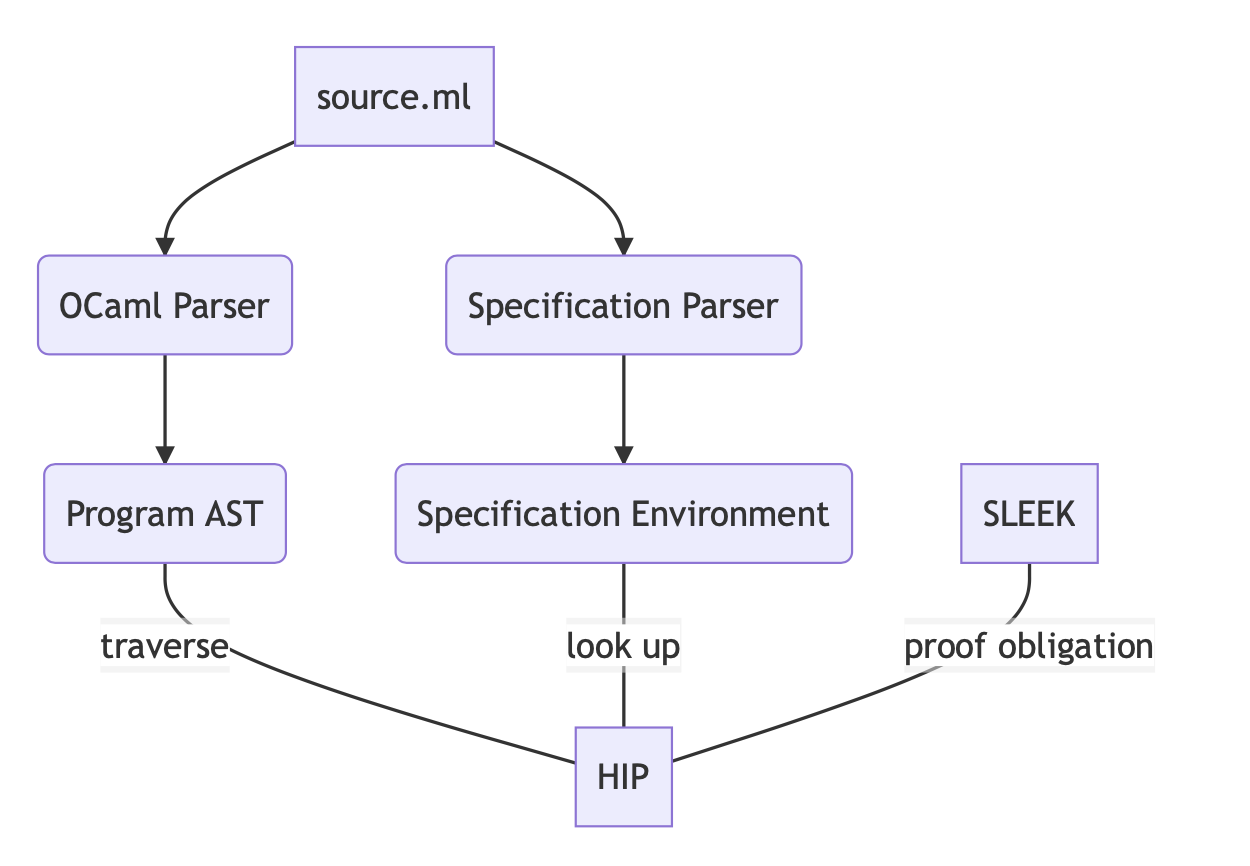
\includegraphics[width=0.8\linewidth]{report/pic/ch-Design/structure.png}
    \caption{Prototype system structure}
    \label{fig:structure}
\end{figure}

\subsection{Front-end Implementation}




\paragraph{OCaml frontend}

\paragraph{Specification syntax}
%talk about nested specification

\paragraph{Specification parser}
%talk about type information



\section{Forward Verification}


\subsection{Logical reasoning rules}

$\Sigma$: context of logical variables. $\Gamma$: context of specifications.

\nameref{rule:fv-method}

\begin{figure}
\centering
\begin{mathpar}
    \inferrule[Fv-Method]{
        \vec{x},\vec{y};P,\mathcal{F}  \provable\hoareabbr{ \Phi_{\text{pre}}}{c}{r}{ \Phi_{\text{post}}}
        \and
        \mathcal{F} =  \textrm{Given } \vec{y}, \Phi_{\text{pre}} \rightarrowtail_{\mathtt{r} } \Phi_{\text{post}}
    } {
        \provable{\texttt{let f=}\lambda \vec{\mathtt{x}}.c \texttt{ where } \mathcal{F} }
    }[]\label{rule:fv-method}
    \\
    \inferrule[Fv-Spec]{
        \Sigma;\Gamma,\mathcal{F} \provable\hoareabbr{ \Delta_1}{c}{r}{ \Delta_2}
    } {
        \Sigma;\Gamma\provable\hoareabbr{\Delta_1\wedge\mathcal{F}}{c}{r}{\Delta_2}
    }[]\label{rule:fv-spec}
    \and
    \inferrule[Fv-Exists]{
        \Sigma,x;\Gamma \provable\hoareabbr{\Delta_1}{c}{r}{\Delta_2}
    } {
        \Sigma;\Gamma\provable\hoareabbr{\exists x.\Delta_1}{c}{r}{\Delta_2}
    }[]\label{rule:fv-exists}
    \\
    \inferrule[Fv-App-Par]{
            \Sigma;\Gamma \provable\hoareabbr{\Delta_0}{{f}}{\texttt{g}}{\Delta_1}
        \and
            \Sigma,\texttt{g};\Gamma \provable\hoareabbr{\Delta_1}{{x}}{\texttt{v}}{\Delta_2}
        \and
            \texttt{g}(\texttt{a},{\mathtt{\vec{b}}}) \ofspec 
                \mathcal{F}
    } {
        \Sigma;\Gamma \provable\hoareabbr{\Delta_0}{f \ {x}}{h}{
            \Delta_2 \wedge
            \texttt{h}({\mathtt{\vec{x'}}}) \ofspec \mathcal{F}[\mathtt{v/a}]
        }
    }[]\label{rule:fv-app-par}
    \\
        \inferrule[Fv-App-Full]{
            \Sigma;\Gamma \provable\hoareabbr{\Delta_0}{{f}}{\texttt{g}}{\Delta_1}
        \and
            \Sigma,\texttt{g};\Gamma \provable\hoareabbr{\Delta_1}{{x}}{\texttt{v}}{\Delta_2}
        \\
            \texttt{g}(\texttt{a}) \ofspec \textrm{Given } \vec{y},
                \Phi_{\text{pre}} \rightarrowtail_{\mathtt{r} } \Phi_{\text{post}} \in \Gamma \cup Spec(\Delta_2)
        \\
            \Delta_2 \entails             
                \Phi_{\text{pre}}(\vec{y})[\mathtt{v/a}]
        \and
            \Phi_{\text{post}}(\vec{y})[\mathtt{v/a,res/r}] \entails \Delta_3
    } {
        \Sigma;\Gamma \provable\hoareabbr{\Delta_0}{f \ {x}}{res}{
            \Delta_3
        }
    }[]\label{rule:fv-app-full}
    \\
    \inferrule[Fv-Match]{
         \Sigma;\Gamma \provable\hoareabbr{\Delta_1}{e}{v}{\Delta_2}
        \and
        \forall i,
             \Sigma, \mathtt{v}, \vec{\mathtt{x}_i} ;\Gamma \provable\hoareabbr{\Delta_2  \wedge
              \mathtt{v}::\texttt{cname}_i\left(\vec{\mathtt{x}_i}\right)}{e_i}{u}{\Delta_3}
    } {
        \Sigma; \Gamma \provable \hoareabbr{\Delta_1}{
            \texttt{match } e \texttt{ with } (\texttt{cname}_i \Rightarrow \lambda \vec{\mathtt{x}_i}.e_i)^*
        }{res}{\Delta_3[\mathtt{res/u}]}
    }[]\label{rule:fv-match}
    \and
    \inferrule[Fv-If]{
        \Sigma;\Gamma \provable\hoareabbr{\Delta_1}{e}{v}{\Delta_2}
        \and
        \Sigma,v;\Gamma \provable \hoareabbr{\Delta_2 \wedge \texttt{v} = \texttt{true}}{e_1}{u}{\Delta_3}
        \and \\
        \Sigma,v;\Gamma \provable \hoareabbr{\Delta_2 \wedge \texttt{v} = \texttt{false}}{e_2}{u}{\Delta_3}
    } {
        \Sigma; \Gamma \provable \hoareabbr{\Delta_1}{
            \texttt{if } e \texttt{ then } e_1 \texttt{ else } e_2 \ 
        }{res}{\Delta_3[\mathtt{res/u}]}
    }[]\label{rule:fv-if}
    \\
    \inferrule[Fv-Cst]{
    } {
        \Sigma; \Gamma \provable \hoareabbr{\Delta}{
          k
        }{res}{\Delta \wedge \texttt{res}=k }
    }[]\label{rule:fv-cst}
    \and
    \inferrule[Fv-Var]{
      \texttt{v} \in \Sigma
      \text{ or }
      \texttt{v}(\vec{x}) = \mathcal{F} \in \Gamma
    } {
        \Sigma; \Gamma \provable \hoareabbr{\Delta}{
          \texttt{v}
        }{res}{\Delta \wedge \texttt{res}= \texttt{v} }
    }[]\label{rule:fv-var}
    \\
    \inferrule[Fv-Fun-Eval]{
      \texttt{v}() = \textrm{Given } \vec{y}, \  \Phi_{\text{pre}} \rightarrowtail_{\mathtt{r} } \Phi_{\text{post}} \in \Gamma
      \and 
      \Delta \provable \Phi_{\text{pre}}(\vec{y})
    } {
        \Sigma; \Gamma \provable \hoareabbr{\Delta}{
          \texttt{v} \ 
        }{res}{\Delta \wedge \texttt{res}=v \wedge 
                \Phi_{\text{post}}(\vec{y})[\mathtt{res/r}] }
    }[]\label{rule:fv-fun-eval}
\end{mathpar}
    \caption{Proof rules of Hoare logic}
    \label{fig:choarelogic}
\end{figure}

Remarks:
\begin{enumerate}
    \item FV-app deals with partial application, which basically creates a new instance of specification for function type. TODO: We did not deal with the separation frame here.
    
    slightly different from the logic defined by yoshida, et al, which uses $m\cdot n=u\{C'\}$ to propagate the verification from an application to its abstraction.  We do the reverse. 
\end{enumerate}


TODO: propose a simple uncurried rule for verifying full application, and prove its correctness based on FV-app partial application rule.

\subsection{Implementation}



\section{Entailment checking}

\subsection{Verification condition encoding}


\subsection{Implementation}



